% !TeX root = 00Main.tex
\section{May: Increase to Four Colonies}

Swarm preparations are most likely in May.
\footnote{Some authorities suggest that it may be possible to have colonies that do not reproduce (swarm).
This is neither desirable or plausible.
It is important to raise new queens each year so we can select for desireable traits.
Furthermore, healthy and unhindered animals should be expected to breed.
So colonies should be expected to swarm.
If a colony does not appear to make swarm preparations in May or June
then you should be suspicious about it's health or genetics.}
This provides an opportunity to raise two new queens.
The intention is to 
begin the month with two colonies on 18 frames each (9Fx9F)
and 
end the month (or June) with four colonies.  
Two new colonies on 11 frames each (11F)
and 
the two original colonies on 5 frames each.\par

\begin{apiary}{Begin with two colonies (and two empty hives)}
    \path (0,0) pic{stand};
    
    \path (4,6) pic{roof};
    \path (4,4) pic{brood=9F};
    \path (4,2) pic{brood=9F};
    \path (4,0) pic{stand};
    
    \path (8,4) pic{roof};
    \path (8,2) pic{brood=2D};
    \path (8,0) pic{stand};

    \path (16,0) pic{stand};
    
    \path (20,6) pic{roof};
    \path (20,4) pic{brood=9F};
    \path (20,2) pic{brood=9F};
    \path (20,0) pic{stand};
    
    \path (24,4) pic{roof};
    \path (24,2) pic{brood=2D};
    \path (24,0) pic{stand};
\end{apiary}

Beside each of the colonies is an empty hive containing two dummy boards.
When swarming begins the old queen will be removed to the empty hive
and
a new queen will be raised in the original hive.
There is an empty hive stand to the other side of each colony
to allow flying bees to be bled off from the old queen's colony
by swapping the hive to the other side of the new queen.

\subsection{Inspect for Swarm Preparations}

The goal of the inspection is to determine if the colony is considering reproducing,
not necessarily that full scale swarm preparations are being made.
So we are looking for queen cells with eggs or grubs.

\begin{figure}[H]
\centering
\begin{tikzpicture}
    \color{white}
    \draw (0, 0) node {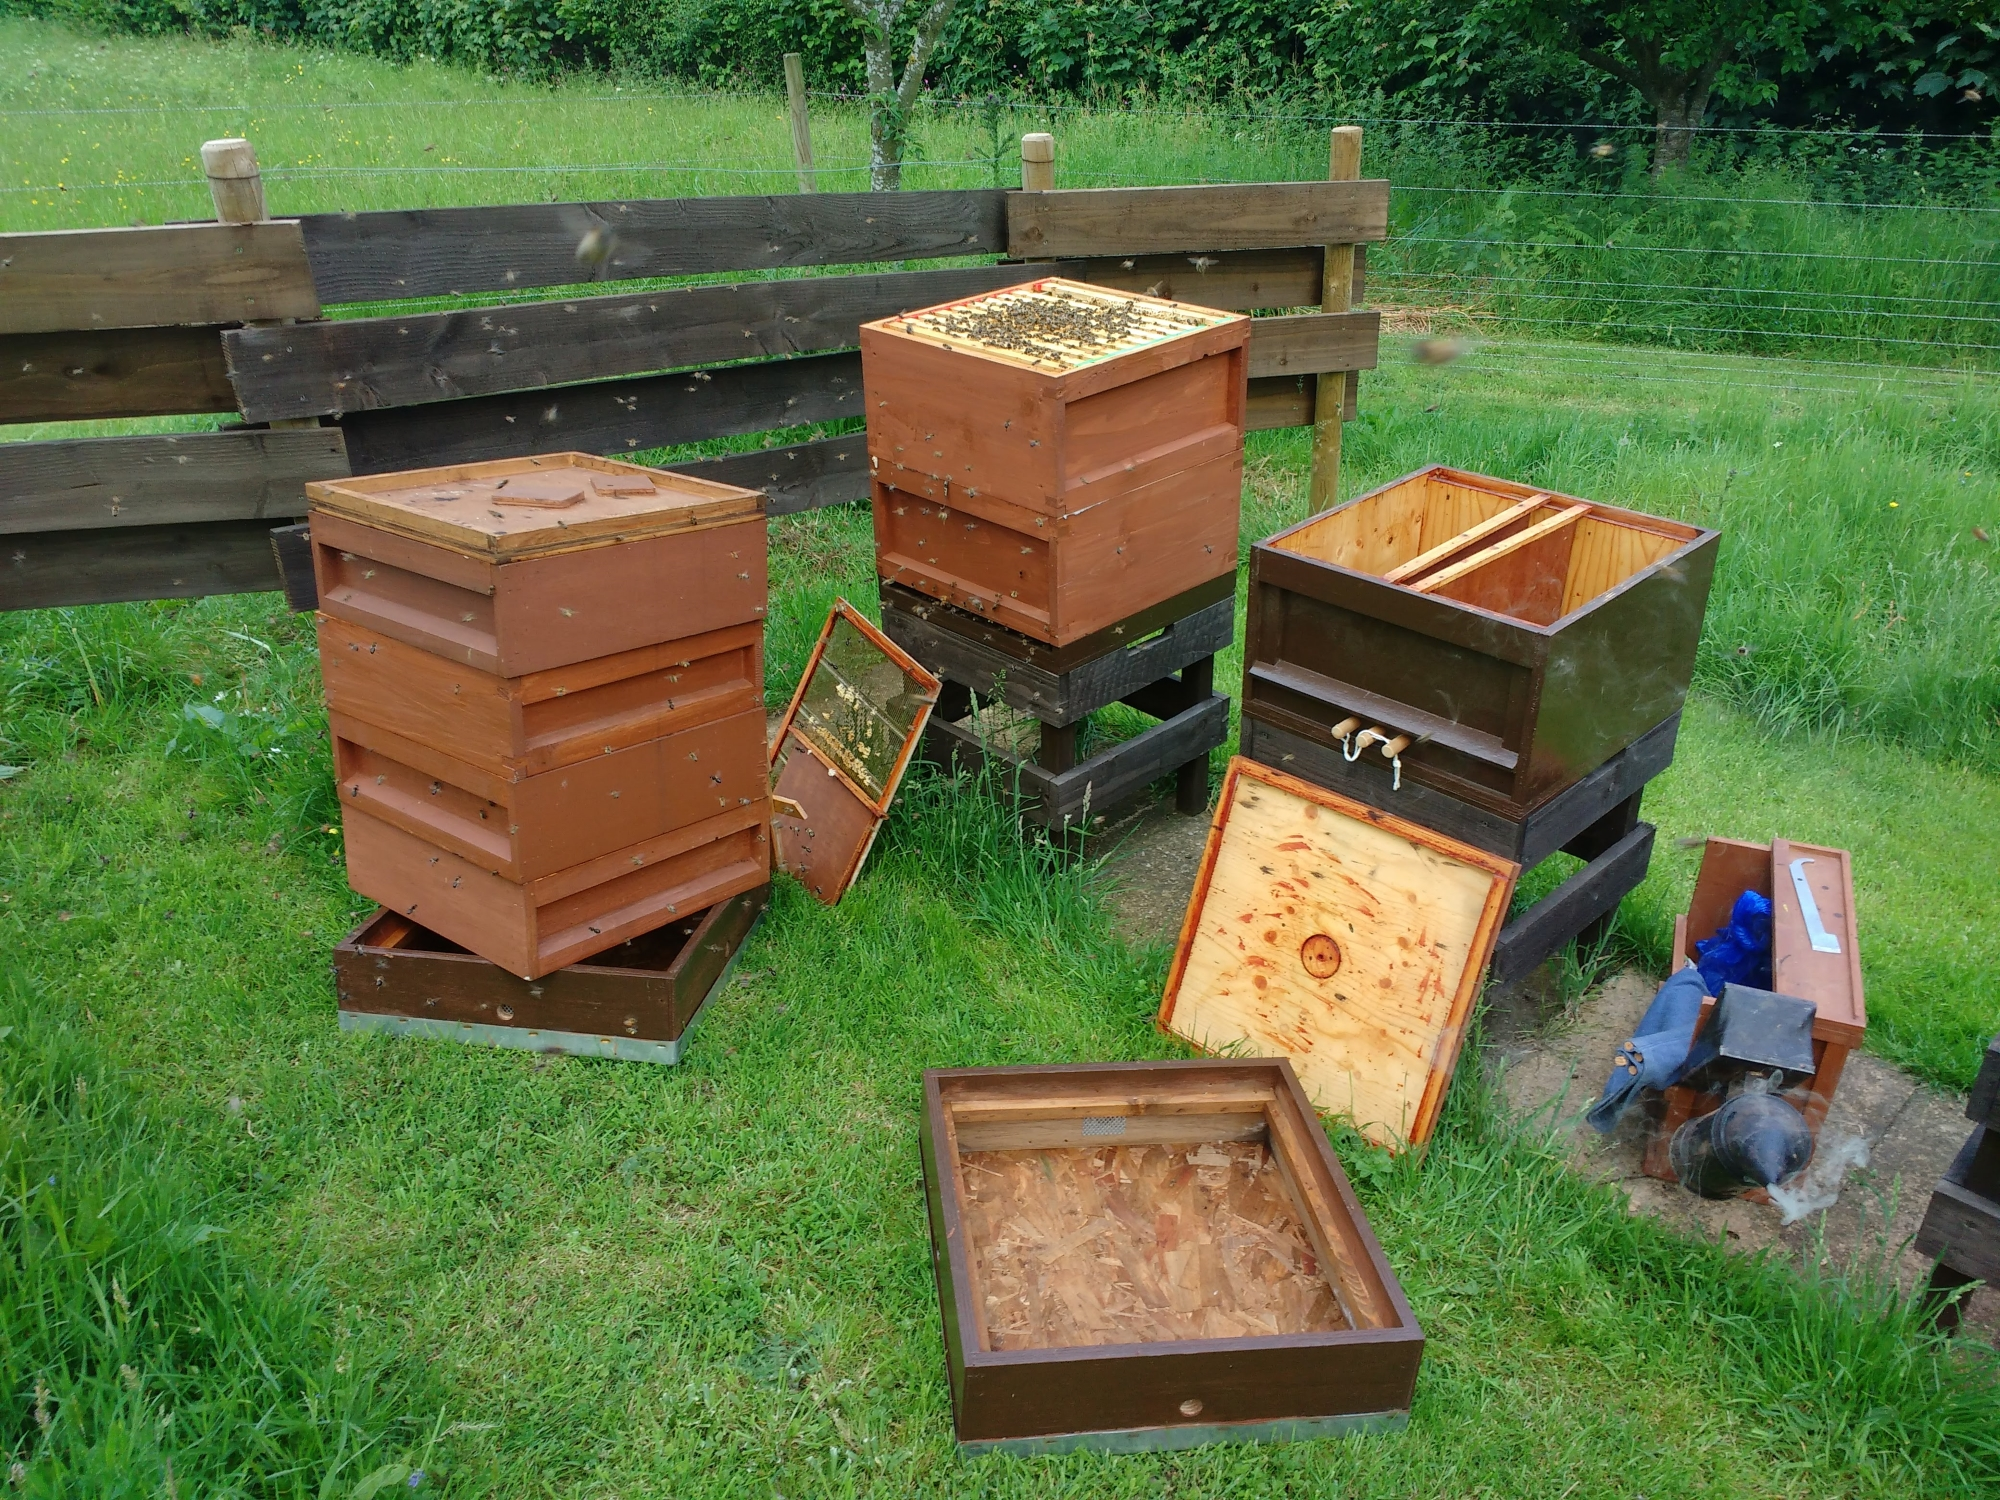
\includegraphics[width=0.9\textwidth]{05MayInspection.jpg}};
    \draw (0, 2) node {Brood Boxes};
    \draw (-3, 0) node {Supers};
    \draw (3, 0.5) node {Spare Brood Box};
\end{tikzpicture}
\caption{Inspect with supers in front of brood, spare brood box to one side}%
\end{figure}

\begin{description}
	\item [Inspect on a 5 to 6 day interval] to give a margin for error.
		From egg to sealed queen cell takes 8 days, so it is possible to inspect on an 8 day interval and many beekeepers use a 7 day interval.
		However, planned inspections can get delayed, maybe rushed or less than through.
		Reduing the inspection interval to 5 to 6 days gives a greater latitude for errors
		in the event that inspections are delayed by weather or unforseen circumstances.
	\item [If you see the queen remove that frame] to the spare brood box even if no swarm preparations are apparent.
		Swarm preparations may not be apparent until later in the inspection.
		Putting the queen aside on a single frame in separate box ensures that she available should it be necessary to split the colony.
		If no swarm preparations are apparent the frame with the queen on can be replaced at the end of the inspection.
\end{description}

\subsection{Plan A: Raise a New Queen}

History as a guide.
If you see queen cells with eggs.
\footnote{Some authorities suggest that you should wait until 
there are queen cells containing grubs.
It is suggested that a queen cell with an egg in might not 
go on to be raised as a queen and that the colony might back out.
This might be possible, but our goal is to raise new queens,
not to avoid reproduction.
So a queen cell containing an egg is sufficient to indicate
that the colony is ready and able to raise a queen.}
Four step approach.

\begin{table}[H]%
\begin{center}
\begin{tabular}{lllcc}
\textbf{Day} & \textbf{Queen} & \textbf{Early Beekeeper} & \textbf{Late Beekeeper} \\
1 & \rdelim\}{3}{3mm}[\textsf{Egg}] & $\leftarrow$ 1. \textbf{Remove queen} \\
2 & & \\
3 & \multirow{2}{*}{\quad $\leftarrow$ Hatching} & \\
\cline{1-1}
4 & \rdelim\}{5}{3mm}[\textsf{Larva}] &  \\
5 \\
6 \\
7 \\
8 & \multirow{2}{*}{\quad $\leftarrow$ Sealing} & $\leftarrow$ 2. \textbf{Cull queen cells} & $\leftarrow$ 1. \textbf{Remove queen} \\
\cline{1-1}
9 & \rdelim\}{8}{3mm}[\textsf{Pupa}] &  \\
10 \\
11 \\
12 \\
13 \\
14 \\
15 & & & $\leftarrow$ 2. \textbf{Cull queen cells} \\
16 & \multirow{2}{*}{\quad $\leftarrow$ Emerging} \\
\cline{1-1}
17 & \rdelim\}{5}{3mm}[\textsf{Maturing}] \\
18 \\
19 \\
20 & & \multicolumn{2}{l}{$\leftarrow$  3. \textbf{Add eggs from original queen}} \\
21 \\
\cline{1-1}
22 & \rdelim\}{4}{3mm}[\textsf{Mating (typical)}] \\
23 \\
24 \\
25 \\
\cline{1-1}
26 & \rdelim\}{2}{3mm}[\textsf{Sperm Transfer}] \\
27 & & \multicolumn{2}{l}{$\leftarrow$  4. \textbf{Check and add eggs from original queen}} \\
\cline{1-1}
28 &   \rdelim\}{7}{3mm}[\textsf{Laying (typical)}] \\
29 \\
30 \\
31 \\
31 \\
33 \\
34  & & \multicolumn{2}{l}{$\leftarrow$  5. \textbf{Check (and maybe add more eggs)}} \\
\end{tabular}
\caption{Swarm Control and Queen Raising}%
\end{center}
\end{table}

Take out the queen to one side along with 7 of the least brood laden frames.  
Add 4 new frames.
Put in a brood box with two dummy boards.
We want the brood to hatch in the production hive.
The queen to one side will be the feeder hive.

The other 11 frames with the queenless hive

\subsubsection*{Step 1: Remove queen}


\begin{quotation}
As soon as occupied queen cells are discovered (eggs or grubs)

Not trying to work out if they are going to swarm.
\begin{description}
  \item[Find queen and remove her], on a frame of (mostly) sealed brood + bees. Remove any queen cells from this frame after checking that there are others in the hive.
	If you can't find her  then guess, she is probably in the middle of the brood nest.
	Then close up the hives and listen.  The noisiest hive is probably queenless.
	Wait and come back in 3 days and look for eggs.
	Put old queen on a stand right beside the stand with the new queen.
	So if there is a problem the two colonies can be united.
  \item[Add four other frames] the ones bearing the least brood so the queen has space to lay.
	These will also be the frames with the most stores which could be useful since most of the flying bees will be lost.
  \item[Remove all queen cells] sealed or otherwise.  There shouldn't be any but sometimes you are late and there are sealed cells.
  \item[Shake in two frames of house bees] because most of the flying bees will be lost and these can be promoted to 
  \item[Add three new brood frames] bringing it up to eight frames.  The winter configuration is 8 on 8.
  
  
Put frame + queen in nucleus.
Add a second frame of mostly sealed brood, if wished + a frame of food + another l or 2
frames of comb (preferably) or foundation.
Shake in sufficient young worker bees to ensure that there are enough to cover the brood.
Close up the nucleus. Put green grass in the entrance if it is to remain in the same apiary.
Check through the parent colony.  Mark frames containing 2 or 3 good, unsealed, queen cells with a drawing pin.
Close up the frames in the brood box and till the remaining space with frames of comb or foundation.
	Remove any sealed queen cells (Although, to use this method, the old queen must still be present so there should not be any.)
  \item[Add 4 new frames and feed] 1:2 syrup to draw out the frames
 \end{description}
\end{quotation}
 
\subsubsection*{Step 2: Cull queen cells}


\begin{quotation}
7 days after the queen was removed.
\begin{description}
  \item[Remove any emergency queen cells] Be meticulous.  Go through it twice.  Brush and smoke, don't shake.
	Go through parent colony and remove any emergency queen cells.  Best to to this three times so every other day.  The last check being a week.
  \item[Keep one (only one) queen cell]
	Select l of the cells previously marked and remove the others.
	Some authorities suggest leaving two, incase one is a dud.
	More than likely you will get a swarm.
	In the event that the one left is a dud the old queen is still available and laying to provide eggs for an emergency queens,
	or to unite back with the colony.
  \item[Add four frames for old queen] The old colony should be building up, add 4 more frames and remove the dummy boards to bring it up to 11 frames.
  \item[Move the old queens colony] to the other side to bleed off bees into the new queens colony.
\end{description}
\end{quotation}

Advantages of the method
Colony remains strong throughout.
Old queen is kept safe and is available if the new queen does not succeed.
The old queen in the nucleus quickly comes back into lay and her brood can be put back into the parent colony.
The method involves minimum time and lifting.
The nucleus is available to use for other procedures later, or can be united back to the original colony.

\subsubsection*{Step 3: Add brood from original queen (optional)}

Some authorities suggest that i
Queen isn't mated and there is increased risk you will squish her or interfere with the mating fly.
However it is an opportunity to keep the number of young bees up.
and will give early warning if the queen was injured.

\begin{description}
  \item[Confirm queen has emerged] look for chewed open.
  \item[Transfer 2 frames between] Brood and eggs to keep strong and to check for
  \item[Restack Supers] so the heavy ones are on top.
  \item[Swap Original hive] to the other side.
\end{description}

\subsubsection*{Step 4: Check and add eggs from original queen}

\begin{description}
  \item[Check transfered frame] look for emergency cells.
  \item[Check queen is laying] 
  \item[Add more eggs and brood] to check queen and if need to deplete origin
\end{description}




